%=======================02-713 LaTeX template, following the 15-210 template==================
%
% You don't need to this template
%
\documentclass[11pt]{article}
\usepackage{amsmath,amssymb,amsthm}
\usepackage{graphicx}
\usepackage{wrapfig}
\usepackage[margin=1in]{geometry}
\usepackage{fancyhdr}
\setlength{\parindent}{0pt}
\setlength{\parskip}{5pt plus 1pt}
\setlength{\headheight}{13.6pt}
\newcommand\question[2]{\vspace{.25in}\hrule\textbf{#1: #2}\vspace{.5em}\hrule\vspace{.10in}}
\renewcommand\part[1]{\vspace{.10in}\textbf{(#1)}}
\newcommand\algorithm{\vspace{.10in}\textbf{Algorithm: }}
\newcommand\correctness{\vspace{.10in}\textbf{Correctness: }}
\newcommand\runtime{\vspace{.10in}\textbf{Running time: }}
\newcommand\tab[1][1cm]{\hspace*{#1}}
\pagestyle{fancyplain}
\lhead{\textbf{\NAME\ (\ANDREWID)}}
\chead{\textbf{HW\HWNUM}}
\rhead{02-713, \today}
\begin{document}\raggedright
%Section A==============Change the values below to match your information==================
\newcommand\NAME{Kadir Emre Otod}  % your name
\newcommand\ANDREWID{150140032}     % your andrew id
\newcommand\HWNUM{2}              % the homework number
%Section B==============Put your answers to the questions below here=======================

% no need to restate the problem --- the graders know which problem is which,
% but replacing "The First Problem" with a short phrase will help you remember
% which problem this is when you read over your homeworks to study.

\question{1}{The First Problem} 

\begin{eqnarray*}
	x(t) & : & non-periodic.  \\
	CTFT & : & x(jw) = \int_{-\infty}^{\infty} x(t) e^{-jwt} dt \\
	& : & x(t) = \dfrac{1}{2\pi} \int_{-\infty}^{\infty} x(jw) e^{jwt} dw
\end{eqnarray*}

\question{2}{The Second Problem} 

\tab \\
\tab \\
\tab \\
\tab \\
\tab \\
\tab \\


\question{3}{The Third Problem} 

\textbf{Unit Impulse} is a sequence which has only one nonzero value, that occurs at n = 0.

\begin{center}
	$\delta[n] =
		\begin{cases}
			1, &         \text{if } n = 0,\\
			0, &         \text{if } n \neq 0.
	\end{cases} $
\end{center}

\textbf{Unit Impulse Response} is the output sequence, when the input to the FIR filter is a unit impulse sequence.

\begin{center}
	$h[n] = \sum_{k=0}^{M}b_k \delta[n-k] = 
	\begin{cases}
	1, &         \text{if } n = 0,\\
	0, &         \text{if } n \neq 0.
	\end{cases}  $
\end{center}


\question{4}{The Fourth Problem} 

There are two general LTI system proporties: \textbf{time invariant} and \textbf{linearity}.

\textbf{Time Invariant:}
\begin{eqnarray*}
	x[n] & \longmapsto & y[n] \\
	x[n-n_0] & \longmapsto & y[n-n_0]
\end{eqnarray*}
\textbf{Linearity:}
\begin{eqnarray*}
	x_1[n] & \longmapsto & y_1[n] \\
	x_2[n] & \longmapsto & y_2[n] \\
	x[n]=\alpha x_1[n]+\beta x_2[n] & \longmapsto & y[n]=\alpha y_1[n]+\beta y_2[n]
\end{eqnarray*}
\textbf{Derivation of Comvolutional Sum:} \\
\tab \\
\tab We can represent any signal as sum of impulses:
\begin{eqnarray*}
	x[n] & \longmapsto & \framebox{S}  \longmapsto y[n] \\
	x[n] & = & \sum_{k=-\infty}^{\infty} x[n]\delta[n-k] \\
\end{eqnarray*}
\tab The output will be:
\begin{eqnarray*}
	y[n] & = & S[x[n]]\\
	y[n] & = & S[\sum_{k=-\infty}^{\infty} x[n]\delta[n-k]] \\
	y[n] & = & \sum_{k=-\infty}^{\infty} x[n]S[\delta[n-k]] \tab \text{(linearity)} \\
\end{eqnarray*}
\tab Now, we need to know $S[\delta[n-k]]$, we can assume that this equation can be written safely:
\begin{eqnarray*}
	h[n] & = & S[\delta[n]]\\
	h[n-k] & = & S[\delta[n-k]] \tab \text{(time invariant)} \\
\end{eqnarray*}
\tab All these equations above give us the convolutional sum formula:
\begin{eqnarray*}
	y[n] & = & \sum_{k=-\infty}^{\infty} x[n]h[n-k] \\
\end{eqnarray*}


\question{5}{The Fifth Problem} 

\part{a} \\
\tab \textbf{Not casual:} The function is dependent on future \\
\tab \textbf{Stable:} x and y can be bounded.

\part{b} \\
\tab \textbf{Casual:} The function is independent on future \\
\tab \textbf{Not stable:} x and y cannot be bounded.

\part{c} \\
\tab \textbf{Casual:} The function is independent on future \\
\tab \textbf{Stable:} The function cannot exceed 1.

\part{d} \\
\tab \textbf{Casual:} The function is independent on future \\
\tab \textbf{Stable:} The function cannot exceed 1.

\cleardoublepage

\question{6}{The Sixth Problem} 

I designed a function named \textbf{my\_conv} which takes two parameters, signal array ($x[n]$) and impulse response ($h[n]$), and returns the convolution.  

\begin{figure}[h]
	\centering
	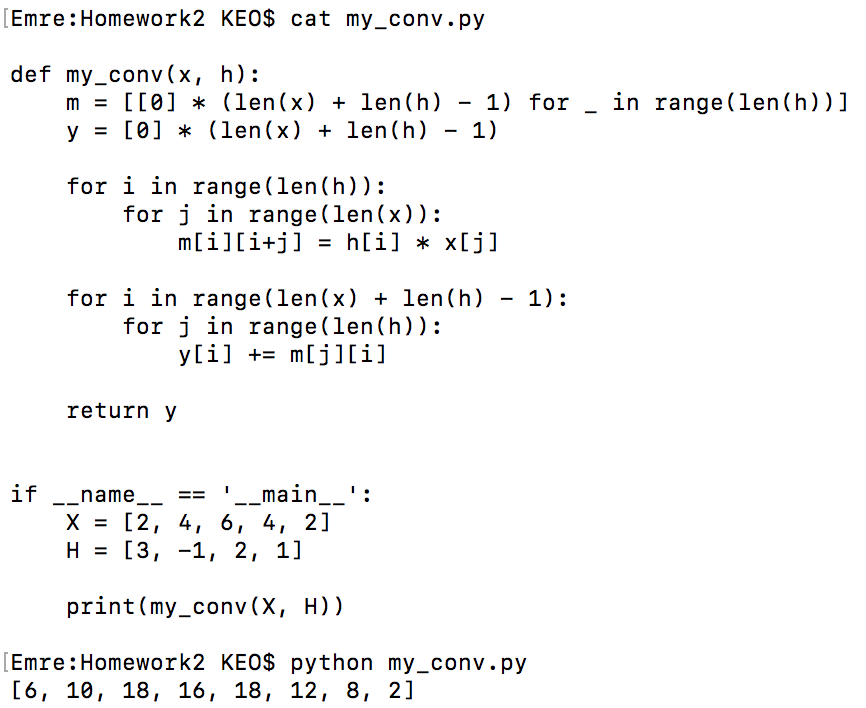
\includegraphics[width=0.7\linewidth]{my_conv}
	\caption{The output of my\_conv function for given parameters in question}
	\label{fig:my_conv}
\end{figure}

\question{7}{The Seventh Problem} 

\begin{eqnarray*}
	y[n] &=& x[n] * h[n] \\
	y[n] &=& 
		\begin{bmatrix}
			2 & 4 & 6 & 4 & 2 \\
		\end{bmatrix} *
		\begin{bmatrix}
			3 & -1 & 2 & 1 & 0 & 0 & 0 & 0 \\
			0 & 3 & -1 & 2 & 1 & 0 & 0 & 0 \\
			0 & 0 & 3 & -1 & 2 & 1 & 0 & 0\\
			0 & 0 & 0 & 3 & -1 & 2 & 1 & 0\\
			0 & 0 & 0 & 0 & 3 & -1 & 2 & 1\\
		\end{bmatrix} \\
	y[n] &=& 
		\begin{bmatrix}
			6 & 10 & 18 & 16 & 18 & 12 & 8 & 2 \\
		\end{bmatrix}
\end{eqnarray*}

\cleardoublepage

\question{8}{The Eighth problem}

The convolve2d method in the scipy library should take at least two parameter, array likes inputs and convolve this two 2-dimensional arrays.

When the program executed, the resulting image, called "result.png" will be created in the very same folder.

\begin{figure}[h]
	\centering
	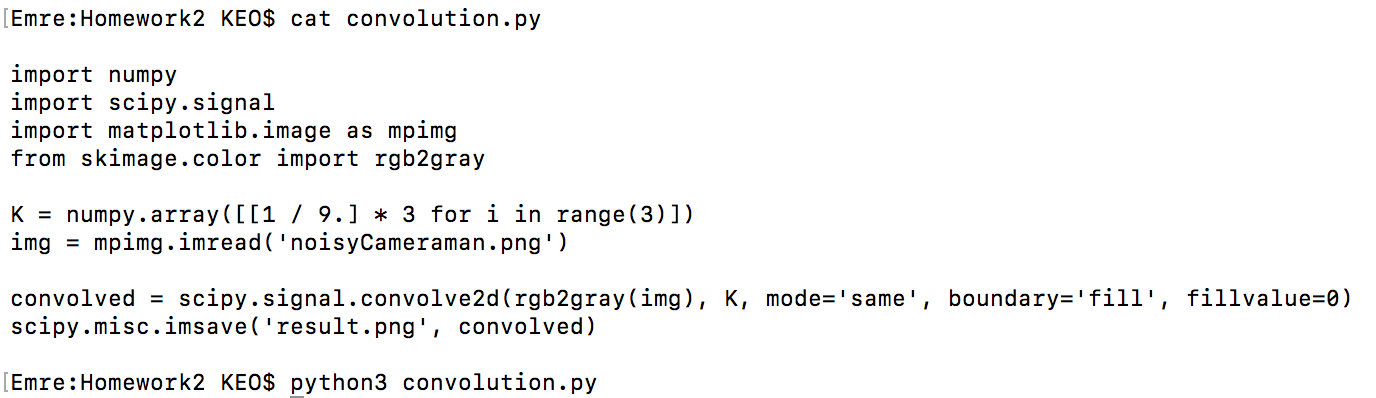
\includegraphics[width=1\linewidth]{convolution}
	\caption{The usage of written python program }
	\label{fig:convolution}
\end{figure}

\begin{figure}[h]
	\centering
	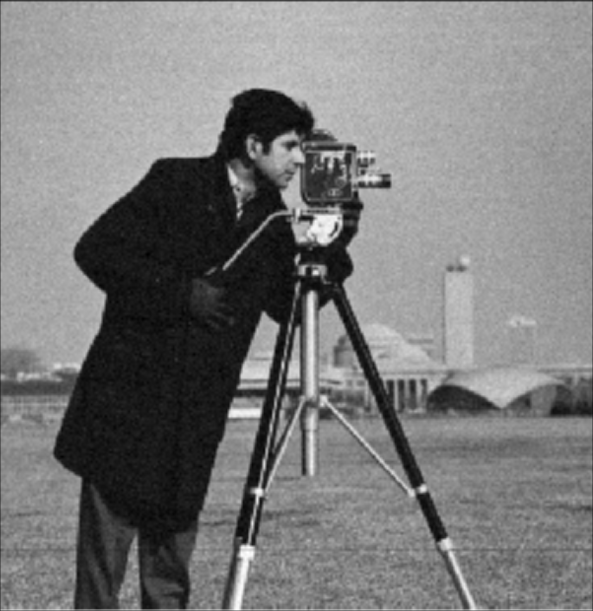
\includegraphics[width=0.5\linewidth]{result}
	\caption{The resulting image }
	\label{fig:result}
\end{figure}

As we can see the resulting image in Figure 3, convolved image is smoother. 


\end{document}
